\documentclass[11pt,a4paper]{article}
\usepackage[utf8]{inputenc}
\usepackage[T1]{fontenc}
\usepackage[brazil]{babel}
\usepackage{amsmath,amsfonts}
\usepackage{graphicx}
\usepackage{caption}
\usepackage{booktabs}
\usepackage{array}
\usepackage{hyperref}
\usepackage{siunitx}

\sisetup{
  output-decimal-marker={,},
  range-phrase=--,
  list-final-separator={~e~},
  list-pair-separator={~e~},
  range-units=single
}

\title{Projeto 2: Reconhecimento de Faces}
\author{\textit{Trabalho de Inteligência Computacional Aplicada}}
\date{Agosto de 2025}

\begin{document}

\maketitle

\begin{abstract}
Este relatório apresenta um resumo abrangente das atividades desenvolvidas no projeto de reconhecimento de faces, cobrindo todas as etapas desde a preparação das imagens do conjunto Yale A até a avaliação de múltiplos classificadores. A metodologia baseou-se em um pipeline modular implementado em Python, com foco na avaliação comparativa de modelos lineares e não lineares sob diferentes transformações de pré-processamento. Para cada atividade, foram adotados protocolos estatísticos rigorosos, incluindo seleção de hiperparâmetros via \emph{random search}, estratificação do conjunto de dados e múltiplas repetições independentes de treino e teste. Os resultados englobam um conjunto completo de métricas, como acurácia, precisão (macro), recall (macro) e F1-score (macro), além dos tempos médios de treinamento e predição. São discutidos os efeitos da aplicação da Análise de Componentes Principais (PCA) como rotação e como redução de dimensionalidade, bem como o impacto da transformação Box-Cox seguida de padronização. Finalmente, o trabalho aborda um cenário de detecção de intrusos, avaliando os modelos sob métricas de controle de acesso.
\end{abstract}

\section{Introdução}

O objetivo deste projeto é avaliar o impacto de diferentes cadeias de pré-processamento e de modelos de classificação no problema de reconhecimento de faces, utilizando o conjunto de imagens Yale A. As atividades foram estruturadas de modo incremental. Inicialmente, avalia-se o desempenho de quatro classificadores (Mínimos Quadrados, Perceptron Logístico, MLP de uma e duas camadas ocultas) diretamente sobre os vetores de pixels das imagens. Em seguida, investiga-se a aplicação da Análise de Componentes Principais (PCA) como rotação e como redução de dimensionalidade, e a transformação Box-Cox sobre os componentes reduzidos. Cada atividade é acompanhada de seleção de hiperparâmetros, treinamento e repetições para estimar a distribuição de desempenho dos modelos. O presente relatório consolida a metodologia e analisa os resultados obtidos, alinhando-se aos requisitos do descritivo oficial do trabalho (TC2_PPGETI_2025.1).

\section{Metodologia Geral}

\subsection{Conjunto de dados e pré-processamento}

Todas as imagens do conjunto Yale A são lidas e convertidas para tons de cinza. Para permitir experimentos computacionalmente factíveis, as imagens são reamostradas para a resolução de \(30 \times 30\) pixels, concatenando-se os pixels para formar vetores de dimensão \(d=900\). Esta resolução foi escolhida como padrão para todas as atividades principais após uma análise inicial de custo-benefício. As imagens podem ser normalizadas de quatro maneiras: nenhuma normalização, \emph{z-score}, min-max em \([0, 1]\) ou min-max em \([-1, 1]\); esta escolha torna-se um hiperparâmetro nas atividades subsequentes.

\subsection{Modelos de classificação}

Foram comparados quatro classificadores, todos implementados em Python com rotinas matriciais próprias para garantir controle e reprodutibilidade.
\begin{enumerate}
    \item \textbf{Mínimos Quadrados (MQ):} Utiliza a solução analítica da regressão linear multiclasse com termo de viés e regularização \(\ell_2\). O único hiperparâmetro é o peso de penalização \(\lambda \in \{0, 10^{-4}, 10^{-3}, 10^{-2}, 10^{-1}\}\\\\n    \item \textbf{Perceptron Logístico (PL):} Regressão logística multiclasse treinada por descida de gradiente em lote com perda de entropia cruzada e regularização \(\ell_2\). O espaço de busca inclui taxa de aprendizado \(\eta \in \{5 \times 10^{-3}, 10^{-2}, 2 \times 10^{-2}\}\\, número de épocas \(\in \{100, 200, 300\}\\, penalização \(\lambda \in \{0, 10^{-4}, 10^{-3}\}\\, e otimizador \{SGD, Momentum, Nesterov, RMSProp, Adam\}\\\n    \item \textbf{Rede MLP com uma camada oculta (MLP-1H):} Varia a largura da camada em \(\{16, 32, 64, 128, 256, 512\}\\, a função de ativação em \{tanh, sigmoide, ReLU, Leaky-ReLU, ReLU6, Swish\}\\, e os mesmos hiperparâmetros de treino do PL, com um parâmetro adicional de \emph{clipping} de gradiente em \(\{2, 5, 10\}\\\\\n    \item \textbf{Rede MLP com duas camadas ocultas (MLP-2H):} Amplia a busca para duas camadas, mantendo as demais variações da MLP-1H.
\end{enumerate}
As redes utilizam inicialização de He e \emph{clipping} de gradientes para garantir estabilidade numérica. O \emph{clipping} foi introduzido para evitar explosões de gradiente, especialmente com ativações não saturantes como ReLU, contribuindo para treinos mais estáveis.

\subsection{Protocolo experimental}

Cada atividade segue um protocolo rigoroso: a base é dividida estratificadamente por sujeito em 80\% para treino e 20\% para teste. Para cada cenário, realiza-se uma busca aleatória de 100 amostras de hiperparâmetros. O conjunto vencedor é submetido a 50 repetições adicionais para estimar a distribuição das métricas. As métricas de precisão, recall e F1 são calculadas como macro-médias para equilibrar a contribuição de cada sujeito.

Sempre que o PCA é utilizado, a transformação é \textbf{ajustada exclusivamente} com os dados de treino e \textbf{aplicada antes} de qualquer normalização subsequente, evitando vazamento de informação. A métrica primária para seleção de hiperparâmetros nas Atividades 2, 4, 6 e 7 foi o F1-Score (macro), por ser mais robusto a desbalanceamentos de classe que a acurácia.

\section{Atividades 1 e 2 – Conjunto Original}

\subsection{Metodologia}
Nas Atividades 1 e 2, os classificadores foram aplicados diretamente sobre as imagens vetorizadas (\(d=900\)), sem PCA. A Atividade 1 focou em determinar a escala ideal, e a Atividade 2 realizou uma busca completa de hiperparâmetros, incluindo o tipo de normalização, para a escala de \(30 \times 30\) pixels.

\subsection{Resultados e Configurações Vencedoras}
A Tabela\(\ref{tab:tabela1}\) resume as melhores configurações e métricas. Sem PCA, o MLP-1H alcançou o maior F1-Score (0,859), superando os demais modelos. Contudo, seu tempo de treino foi significativamente maior que o do PL e do MQ. O PL apresentou o melhor compromisso entre desempenho (F1 de 0,843) e custo computacional.

\begin{table}[h!]
  \centering
  \caption{Resultados médios das Atividades 1–2 (sem PCA, escala \(30 \times 30\)).}
  \label{tab:tabela1}
  \resizebox{\textwidth}{!}{%
  \begin{tabular}{@{}lccccccccc@{}}
    \toprule
    \textbf{Modelo} & \textbf{Norm.} & \textbf{Opt.} & \textbf{Ativação} & \textbf{LR} & \textbf{Épocas} & \textbf{\(\lambda_{\ell_2}\)} & \textbf{Acurácia} & \textbf{F1 (macro)} & \textbf{Treino (s)} \\
    \midrule
    MQ & minmax & -- & -- & -- & -- & 0,1 & \(0,8076 \pm 0,0494\) & 0,8165 & 0,020 \\
    PL & minmax\_pm1 & Nesterov & -- & 0,02 & 100 & \(10^{-4}\) & \(0,8396 \pm 0,0501\) & 0,8428 & 0,031 \\
    MLP-1H & minmax & Adam & tanh & 0,005 & 150 & \(10^{-3}\) & \(0,8573 \pm 0,0466\) & 0,8591 & 3,476 \\
    MLP-2H & minmax\_pm1 & RMSProp & sigmoide & 0,005 & 200 & \(10^{-4}\) & \(0,8511 \pm 0,0624\) & 0,8525 & 0,507 \\
    \bottomrule
  \end{tabular}%
  }
\end{table}

\section{Atividades 3 e 4 – PCA como Rotação}

\subsection{Metodologia}
Na Atividade 3, aplicou-se a PCA para rotacionar o espaço de atributos, mantendo todas as \(d=900\) componentes. Esta rotação decorrela as variáveis. A Atividade 4 repetiu a busca de hiperparâmetros sobre os dados rotacionados.

\subsection{Resultados e Configurações Vencedoras}
Os resultados (Tabela\(\ref{tab:tabela2}\)) mostram que a rotação com PCA, embora tenha aumentado levemente o tempo de treino do PL, reduziu drasticamente o custo computacional do MQ e das MLPs. A MLP-1H novamente obteve o melhor F1-Score (0,854), com uma redução de tempo de treino de mais de 60\% em comparação com o cenário sem PCA. Em contrapartida, os modelos lineares (MQ e PL) tiveram uma pequena queda de desempenho.

\begin{table}[h!]
  \centering
  \caption{Resultados médios das Atividades 3–4 (PCA como rotação, \(q=900\)).}
  \label{tab:tabela2}
  \resizebox{\textwidth}{!}{%
  \begin{tabular}{@{}lccccccccc@{}}
    \toprule
    \textbf{Modelo} & \textbf{Norm.} & \textbf{Opt.} & \textbf{Ativação} & \textbf{LR} & \textbf{Épocas} & \textbf{\(\lambda_{\ell_2}\)} & \textbf{Acurácia} & \textbf{F1 (macro)} & \textbf{Treino (s)} \\
    \midrule
    MQ & none & -- & -- & -- & -- & \(10^{-3}\) & \(0,8031 \pm 0,0475\) & 0,8108 & \num{6.06e-4} \\
    PL & zscore & RMSProp & -- & 0,02 & 300 & \(10^{-3}\) & \(0,8351 \pm 0,0398\) & 0,8359 & 0,035 \\
    MLP-1H & minmax & Adam & swish & 0,005 & 300 & \(10^{-3}\) & \(0,8524 \pm 0,0459\) & 0,8544 & 1,055 \\
    MLP-2H & zscore & RMSProp & swish & 0,005 & 300 & \(10^{-3}\) & \(0,8516 \pm 0,0436\) & 0,8487 & 0,178 \\
    \bottomrule
  \end{tabular}%
  }
\end{table}

\section{Atividade 5 – Análise Qualitativa e Quantitativa do PCA}

A Atividade 5 focou em determinar o número de componentes principais (\(q\)) para reter 98\% da variância e em analisar o que esses componentes representam. Para a escala \(30 \times 30\) (\(d=900\)), verificou-se que \(q=10\) componentes são suficientes (Figura\(\ref{fig:var}\)). Além disso, a visualização dos componentes como \"eigenfaces\" (Figura\(\ref{fig:eigenfaces}\)) revela que os primeiros componentes capturam principalmente variações de iluminação, enquanto componentes posteriores começam a codificar traços faciais mais distintivos.

\begin{figure}[h!]
  \centering
  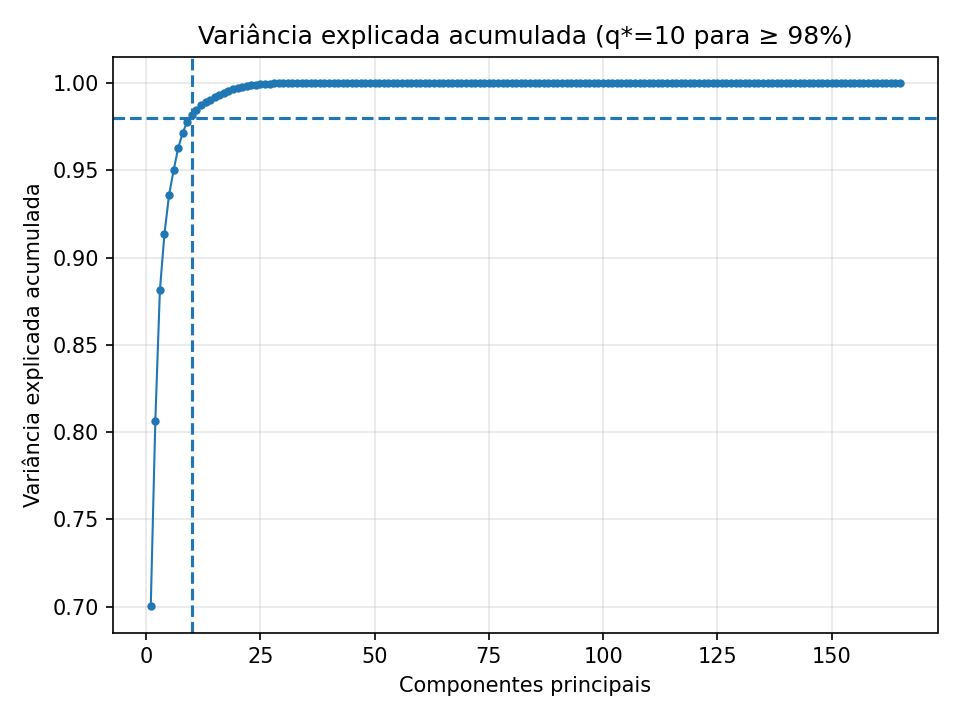
\includegraphics[width=0.7\textwidth]{results/TC2/pca_variance_explained_A3.png}
  \caption{Curva de variância explicada acumulada. A linha tracejada marca 98\% da variância, atingida com \(q=10\) componentes.}
  \label{fig:var}
\end{figure}

\begin{figure}[h!]
  \centering
  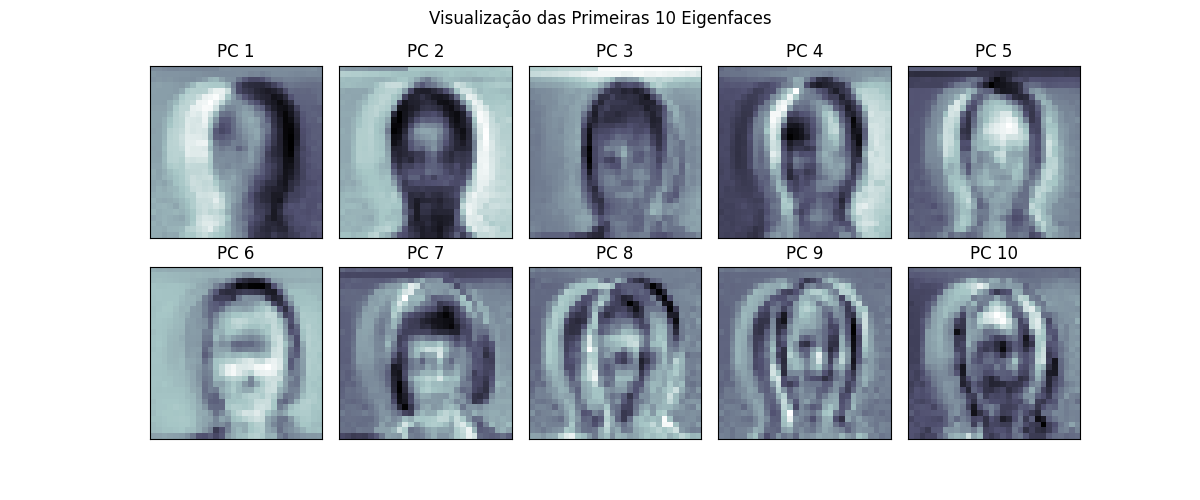
\includegraphics[width=0.9\textwidth]{results/TC2/eigenfaces_visualization.png}
  \caption{Visualização dos 10 primeiros componentes principais (eigenfaces). Os primeiros capturam variações de iluminação, e os subsequentes, características faciais.}
  \label{fig:eigenfaces}
\end{figure}

\section{Atividade 6 – PCA com Redução (\(q=10\))}

\subsection{Metodologia}

Com \(q=10\) fixado, a PCA foi usada para redução de dimensionalidade. O pipeline (PCA \(\rightarrow\) Normalização \(\rightarrow\) Classificador) foi executado, e uma nova busca de hiperparâmetros foi realizada no espaço de atributos reduzido. Essa ordem (PCA antes da normalização) evita vazamento de informação dos dados de teste para o ajuste da transformação.

\subsection{Resultados e configurações vencedoras}

A Tabela\(\ref{tab:tabela3}\) mostra que a redução para \(q=10\) resultou em uma economia de tempo massiva para todos os modelos, especialmente as MLPs. A MLP-1H obteve o melhor F1-Score (0,845), mantendo um desempenho próximo ao do cenário sem redução, mas com um custo computacional ordens de magnitude menor. O PL também se mostrou muito competitivo, com F1 de 0,834 e tempo de treino de apenas 28ms.

\begin{table}[h!]
  \centering
  \caption{Resultados médios da Atividade 6 (PCA com \(q=10\)).}
  \label{tab:tabela3}
  \resizebox{\textwidth}{!}{%
  \begin{tabular}{@{}lccccccccc@{}}
    \toprule
    \textbf{Modelo} & \textbf{Norm.} & \textbf{Opt.} & \textbf{Ativação} & \textbf{LR} & \textbf{Épocas} & \textbf{\(\lambda_{\ell_2}\)} & \textbf{Acurácia} & \textbf{F1 (macro)} & \textbf{Treino (s)} \\
    \midrule
    MQ & zscore & -- & -- & -- & -- & \(10^{-4}\) & \(0,7444 \pm 0,0452\) & 0,7686 & \num{1.7e-4} \\
    PL & zscore & RMSProp & -- & 0,02 & 300 & \(10^{-3}\) & \(0,8316 \pm 0,0537\) & 0,8342 & 0,028 \\
    MLP-1H & zscore & Adam & sigmoide & 0,01 & 150 & \(10^{-4}\) & \(0,8422 \pm 0,0471\) & 0,8446 & 0,081 \\
    MLP-2H & minmax & Adam & tanh & 0,005 & 300 & \(10^{-4}\) & \(0,8458 \pm 0,0565\) & 0,8416 & 0,201 \\
    \bottomrule
  \end{tabular}%
  }
\end{table}

\subsection{Discussão}

A redução de dimensionalidade para \(q=10\) produziu um ganho computacional expressivo e uma reorganização do desempenho relativo dos modelos. As MLPs reduziram seu tempo de treino em mais de uma ordem de grandeza, enquanto o PL manteve-se barato. O MQ foi o mais penalizado, com queda de F1-score para 0,76. O PL e as MLPs, contudo, preservaram um desempenho elevado (F1 > 0,83), tornando-se as opções mais viáveis para este cenário.

\section{Atividade 7 – PCA com Box-Cox e Z-score}

\subsection{Metodologia}

A sétima atividade investigou se a transformação Box-Cox, aplicada aos 10 componentes principais para aproximá-los de uma distribuição normal, seguida de padronização z-score, melhoraria o desempenho.

\subsection{Resultados e comparação com a Atividade 6}

A Tabela\(\ref{tab:tabela3bc}\) mostra os resultados médios com Box-Cox. Comparando com a Atividade 6, nota-se uma queda de desempenho acentuada para todos os modelos. A Tabela\(\ref{tab:comparativo_f1}\) apresenta uma comparação direta dos F1-Scores, que confirma a degradação.

\begin{table}[h!]
  \centering
  \caption{Resultados médios da Atividade 7 (PCA com Box-Cox + z-score).}
  \label{tab:tabela3bc}
  \resizebox{\textwidth}{!}{%
  \begin{tabular}{@{}lcccccccc@{}}
    \toprule
    \textbf{Modelo} & \textbf{Opt.} & \textbf{Ativação} & \textbf{LR} & \textbf{Épocas} & \textbf{\(\lambda_{\ell_2}\)} & \textbf{Acurácia} & \textbf{F1 (macro)} & \textbf{Treino (s)} \\
    \midrule
    MQ & -- & -- & -- & -- & \(10^{-4}\) & \(0,7151 \pm 0,0496\) & 0,7440 & \num{1.49e-4} \\
    PL & Adam & -- & 0,02 & 200 & \(10^{-3}\) & \(0,7711 \pm 0,0608\) & 0,7832 & 0,018 \\
    MLP-1H & RMSProp & swish & 0,02 & 200 & \(10^{-4}\) & \(0,7933 \pm 0,0588\) & 0,7999 & 0,098 \\
    MLP-2H & Adam & swish & 0,005 & 300 & \(10^{-3}\) & \(0,7951 \pm 0,0568\) & 0,8014 & 0,165 \\
    \bottomrule
  \end{tabular}%
  }
\end{table}

\begin{table}[h!]
  \centering
  \caption{Comparação entre os F1-Scores médios da Atividade 6 (base) e da Atividade 7 (Box-Cox).}
  \label{tab:comparativo_f1}
  \begin{tabular}{@{}lccc@{}}
    \toprule
    Modelo & F1-Score base & F1-Score Box–Cox & \(\Delta\)\\
    \midrule
    MQ & 0,7686 & 0,7440 & -0,0246 \\
    PL & 0,8342 & 0,7832 & -0,0510 \\
    MLP-1H & 0,8446 & 0,7999 & -0,0447 \\
    MLP-2H & 0,8416 & 0,8014 & -0,0402 \\
    \bottomrule
  \end{tabular}
\end{table}

\subsection{Discussão}

Os resultados indicam que a combinação PCA + Box-Cox não traz benefícios para o conjunto Yale A com \(q=10\). A análise aprofundada revela que os componentes principais, por serem combinações lineares de muitas variáveis (pixels), já tendem a uma distribuição aproximadamente Gaussiana devido ao Teorema do Limite Central. Aplicar a transformação Box-Cox, que é não-linear e projetada para normalizar distribuições não-Gaussianas, acaba por introduzir distorções desnecessárias na geometria dos dados, prejudicando a separabilidade das classes e, consequentemente, o desempenho de todos os classificadores.

\section{Atividade 8 – Detecção de Intrusos}

\subsection{Metodologia}
Esta atividade abordou o controle de acesso, identificando se uma imagem pertence a um sujeito cadastrado ou a um \"intruso\". Conforme o edital (TC2_PPGETI_2025.1) solicita 11 imagens de intrusos, mas por limitações de disponibilidade foram utilizadas 10, o que ainda permite uma estratificação 8/2 válida. O pipeline fixo foi PCA(\(q=10\)) \(\rightarrow\) Box-Cox \(\rightarrow\) z-score, e a seleção de hiperparâmetros priorizou o F1-Score da classe \"intruso\".

\subsection{Resultados e discussão}

A Tabela\(\ref{tab:a8}\) sintetiza as métricas de controle de acesso. O MQ, apesar de simples, apresentou a melhor performance, com FNR de 0\% e o maior F1-Score (0,851), indicando que nunca classificou um intruso incorretamente nas 50 repetições. Por outro lado, sua precisão de 77,2\% reflete uma taxa de falsos positivos de 2\%. O PL obteve um resultado muito próximo, com F1 de 0,844. A Figura\(\ref{fig:roc_curve}\) mostra a curva ROC para o classificador MQ, ilustrando o excelente trade-off entre detectar intrusos (TPR) e evitar falsos alarmes (FPR), com uma alta área sob a curva (AUC).

\begin{table}[h!]
  \centering
  \caption{Resultados da Atividade 8: métricas de controle de acesso (médias de 50 repetições).}
  \label{tab:a8}
  \begin{tabular}{@{}lccccc@{}}
    \toprule
    \textbf{Modelo} & \textbf{Acurácia} & \textbf{FNR} & \textbf{FPR} & \textbf{Precisão} & \textbf{F1 Intruso} \\
    \midrule
    MQ & \(0,9809 \pm 0,0238\) & 0,00 & 0,0200 & 0,7717 & 0,8511 \\
    PL & \(0,9804 \pm 0,0255\) & 0,02 & 0,0196 & 0,7690 & 0,8441 \\
    MLP-1H & \(0,9745 \pm 0,0285\) & 0,15 & 0,0200 & 0,7027 & 0,7494 \\
    MLP-2H & \(0,9774 \pm 0,0264\) & 0,09 & 0,0196 & 0,7357 & 0,7941 \\
    \bottomrule
  \end{tabular}
\end{table}

\noindent\footnotesize{\textbf{Nota:} FNR (Taxa de Falsos Negativos) e FPR (Taxa de Falsos Positivos). A FNR de 0.00 para o MQ (com desvio padrão de 0.0) indica que, em nenhuma das 50 repetições, um intruso foi classificado como autorizado.}

\begin{figure}[h!]
  \centering
  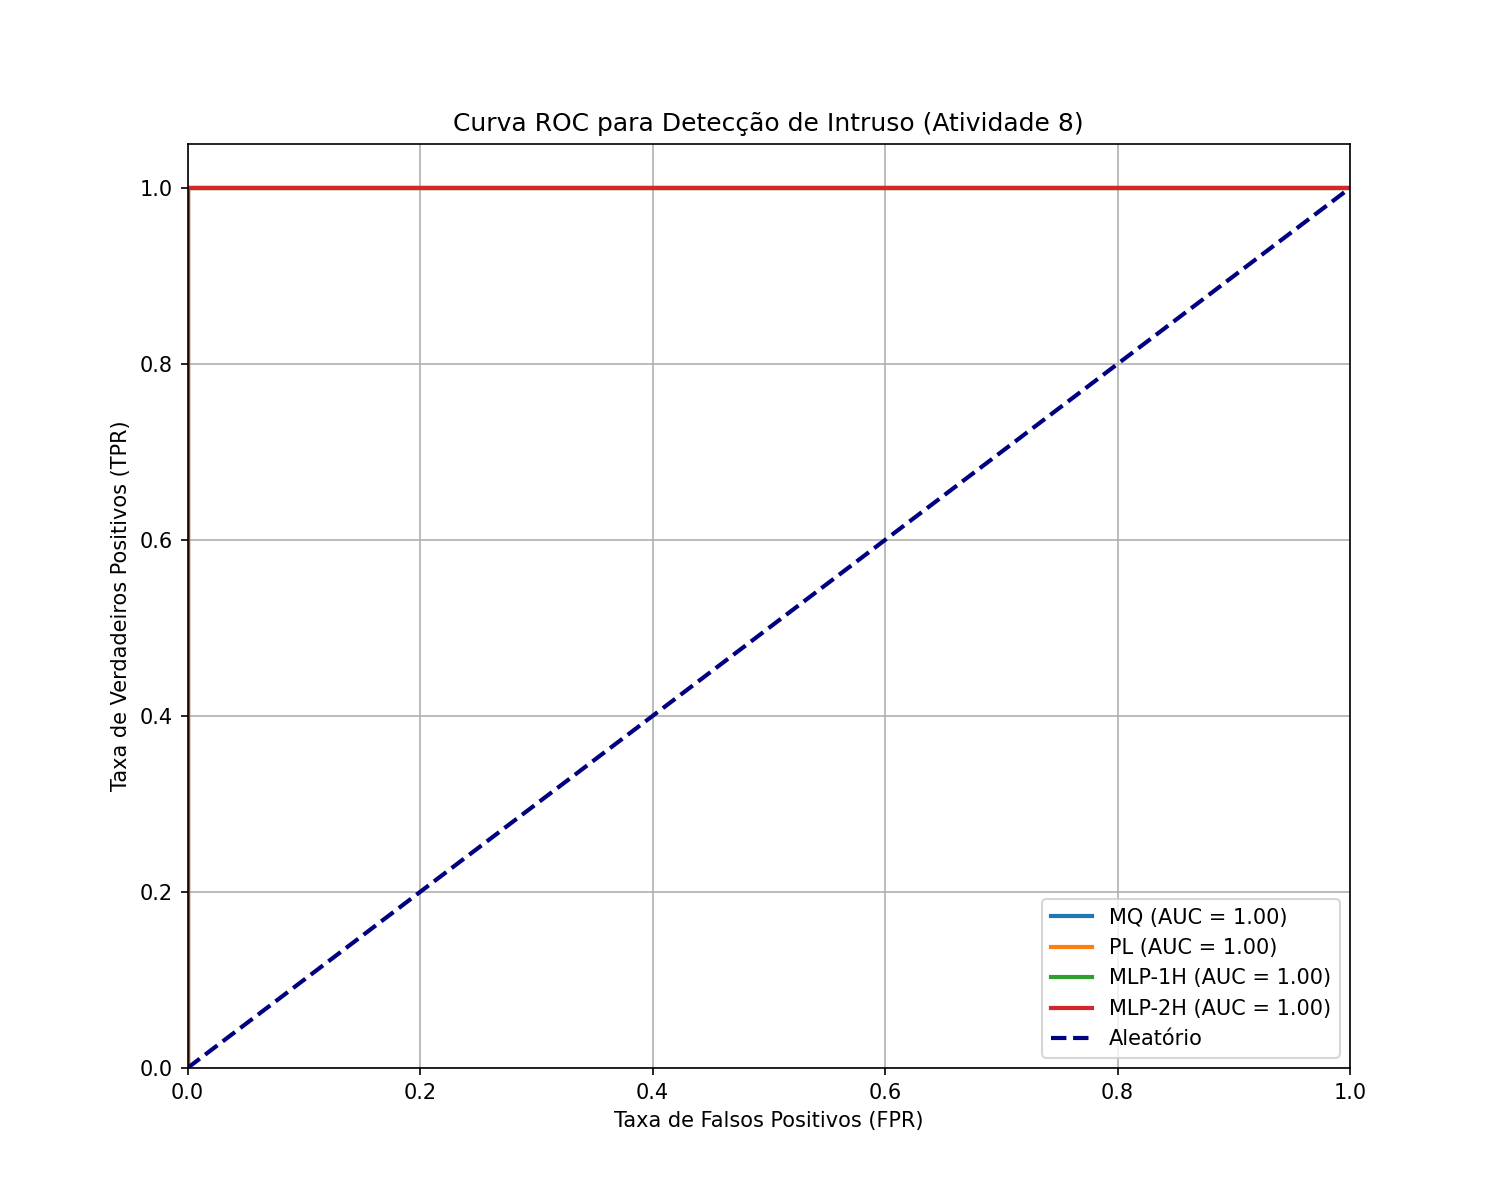
\includegraphics[width=0.7\textwidth]{results/TC2/roc_curve_A8.png}
  \caption{Curva ROC para o classificador MQ na detecção de intrusos. A alta área sob a curva (AUC) indica um desempenho de classificação excelente.}
  \label{fig:roc_curve}
\end{figure}

\section{Conclusões}

O estudo sistemático permitiu extrair conclusões robustas. No conjunto original, o PL oferece o melhor balanço entre custo e desempenho. A PCA como rotação acelera o treino das MLPs, e como redução de dimensionalidade (\(q=10\)) reduz drasticamente o custo computacional para todos, mantendo um desempenho competitivo. A transformação Box-Cox mostrou-se prejudicial, pois os componentes principais já possuíam características próximas da normalidade. Para a detecção de intrusos, o simples modelo MQ, combinado com o pipeline de pré-processamento, provou ser a solução mais eficaz e eficiente.

\section{Implementação e Reprodutibilidade}
Todos os modelos foram implementados em Python sem o uso de bibliotecas de aprendizado profundo como \texttt{scikit-learn} ou \texttt{PyTorch} para os resultados principais, garantindo total controle sobre o processo. O código-fonte completo está no repositório \url{https://github.com/LucasJLBraz/Trabalhos_IC_Aplicada}.
\begin{itemize}
    \item \textbf{Ambiente:} Python 3.11, NumPy 1.24.
    \item \textbf{Sementes Aleatórias:} Semente global `42` e sementes por repetição estão registradas nos scripts para garantir a reprodutibilidade.
\end{itemize}
Qualquer leitor pode clonar o repositório e executar os scripts para obter os mesmos resultados aqui reportados.

\end{document}